\documentclass[12pt]{report}
\usepackage[utf8]{inputenc}
\usepackage{hyperref}
\usepackage{makecell}
\usepackage{paralist}
\usepackage{longtable}
\usepackage{tabularx}
\usepackage{tikz}
\usepackage{Ausarbeitung}

\author{Florens Werner, Bastian Hofmann \\ Technische Universität München}

\title{ENIAC, IAS, EDVAC und EDSAC: Die ersten Röhrenrechner in den USA und GB}

\date{04.05.2016}

\begin{document}

\maketitle

\begin{abstract}
TODO Einführung - Jetzt new
\end{abstract}

\section{IAS Machine}

\subsection{Geschichte}


Die Maschine basiert auf John von Neumanns Arbeit ``Preliminary Discussion of the
Logical Design of an Electronic Computing Instrument'' und wurde, unter seiner Aufsicht, 
am Institute for Advanced Studies (IAS) in Princeton, New Jersey entwickelt.
Mit der Entwicklung wurde 1945 begonnen und der Computer wurde 1951 fertiggestellt.
Bis zu diesem Zeitpunkt wurden Universalrechner hauptsächlich für militärische Zwecke verwenden,
zum Beispiel um Flugbahnen von Artilleriegeschossen zu berechnen.
Nun wurde erstmals ein Universalrechner an einer Universität entwickelt, der dazu gedacht war
wissenschaftliche Erungenschaften zu ermöglichen.
Dieses Konzept führte unter anderem dazu, dass sämtliche Dokumente, Beschreibungen der Maschine und Schaltpläne veröffentlicht
wurden. Auf Grundlage dieser Dokumente konnten Universitäten auf der ganzen Welt ihre eigenen IAS Maschinen
bauen. Auch die Programmierbare Elektronische Rechenmaschine München (PERM), die in der Informatikabteilung des Deutschen Museums 
in München ausgestellt ist eine solche IAS Maschine.\\

Die Architektur die in dem oben genannten Bericht erläutert wird, wird Heute allgemein 
Von-Neumann-Architektur genannt obwohl John von Neumann nur einer der Verfasser der Abhandlung ist.
Neben John von Neumann haben auch Arthur Burks und Herman Goldstine an der Architektur gearbeitet. 
Es ist davon auszugehen, dass die Architektur wesentlich von John von Neumann 
beeinflusst wurde und deshalb nach ihm benannt ist.

\subsection{Technische Beschreibung}

Im folgenden möchte ich näherer auf Aufbau, Funktionsweise und Architektur des Computers eingehen. Und einen groben Überblick über
die einzelnen Bausteine geben, aus denen die IAS Maschine besteht. Es ist bereits bekannt, dass ein Computer der eine Von-Neumann-Architektur 
besitzt aus vier wesentlichen Bausteinen besteht: Speicherwerk, Rechenwerk, Ein-/Ausgabewerk und dem Steuerwerk. Diese vier Bausteine sind
auch in der IAS Maschine zu finden in werden in der Abhandlung von John von Neumann beschrieben.

Zunächst werden aber allgemeine Eigenschaften der Maschine beschrieben.

\subsubsection{Zahlenrepresentation}

Man entschied sich für eine Wortbreite von 40Bit, da diese Wortbreite für die meisten geplanten Anwendungen ausreichend war. Es konnten aber in der Theorie mehrere
Wörter als eine Zahl interpretiert werden. Somit war man in der Lage mit sehr viel grösseren Zahlen zu rechnen.
Bei der Planung der Maschine wurde angenommen, dass die meisten Zahlen, die verarbeitet werden sollen zwischen -1 und 1 liegen.
Deshalb wurde eine Kodierung gewählt, die die 40 Bit von links nach rechts zu Vorzeichenbit, gefolgt von $2^{-1}$, $2^{-2}$, ... $2^{-39}$ kodiert.
Wie gewohnt wird das Vorzeichenbit mit $0$ für eine positive und $1$ für eine negative Zahl kodiert.
Tatsächlich ist diese Kodierung aber mehr eine Konvention antstatt eine tatsächliche Eigenschafft der Maschine. Die Konvention wird nur bei der 
Multiplikation und Division tatsächlich so gefordert. Bei Addition und Substraction kann der Programmierer seine eigene Kodierung wählen und so
zum Beispiel auch mit Intigern rechnen, indem der die 40 Bit als $2^{39}$, $2^{38}$, ... $2^{0}$ betrachtet. Der Wertebereich beträgt dann $[0,1099511627776]$.

\subsubsection{Speicherwerk}

Natürlich wäre es optimal wenn man für den Speicher eine Reihe von Registern die aus Elektornenröhren-Flip-Flops bestehen zur Verfügung hätte. Da man dann aber dazu aber $40n$ Flip-Flops, für $n$ Speicherwörter benötigen würde und $n$ möglichst groß sein soll, hat man sich für Quecksilberröhren entschieden.\\
Für den Speicher war eine Größe von etwa 4000 Wörtern geplant. Dafür wurden 40 solcher Röhren benötigt. Diese Eigenschaft des Speichers hatte eine weitere wichtige Eigenschaft. Da die Wortbreite des Computers 40Bit betrug, konnte man in einem Schritt ein ganzes Wort aus dem Speicher lesen, indem man einfach je ein Bit aus jeder Röhre las. Somit hatte man die Möglichkeit eine parallele Maschine zu bauen und musste nicht jedes Bit seriell, wie bei vorherigen Maschinen (zum Beispiel EDVAC), ein Bit nach dem andereren verrechnen.\\
Zwischen Speicherwerk und Rechenwerk gibt es eine Art Puffer, das Selectronregister. Dort werden die aus dem Speicher kommen hinein geladen bevor sie in das Rechenwerk gehen. Andersherum funktioniert das laden von Werten aus dem Rechenwerk in den Speicher analog.

\subsubsection{Rechenwerk}

In der Recheneinheit der IAS Maschine gibt es zwei für den Programmierer benutzbare Register: Den Akkumulator und das Multiplikationsregister.
Der Akkumulator ist eine paralelle Speichereinheit die eine Zahl empfangen kann und diese auf die gespeicherte Zahl addieren kann. Um eine solche
binäre Addition durchzuführen werden zwei Schritte benötigt.\\
Im ersten Schritt werden die Zahlen übereinander gelegt und jedes Paar von Bits addiert. Im zweiten Schritt werden die Carries die im ersten Schritt entstehen behandelt.
Die Carries müssen nacheinander behandelt werden, da ein Carry ein zweites auslösen kann. Schlimmstenfalls werden so 39 Carries ausgelöst.
Substraktion wird durch Umwandlung der Zahl ins Zweierkomplement und anschließender Addition umgesetzt.
Außerdem kann das Rechenwerk Multiplizieren und Dividieren.

\subsubsection{Steuerwerk}

Wie in der von Neumann-Architektur festgelegt, soll das auszuführende Programm zusammen mit den Daten im Speicher stehen. Um das Programm zu beschreiben, waren zwei Typen von Befehlen geplant. Ein Befehl des ersten Typs holt erst einen Wert aus einer bestimmten Stelle im Speicher in das Selectronegister und wendet dann eine Funktion des Rechenwerks darauf an. Ein Befehl des zweiten Typs holt einen Wert aus dem Rechenwerk in das Selectronregister und lädt im zweiten Schritt den Inhalt des Selectronregisters in eine gegebene Stelle im Speicher. Außerdem gibt es bedingte Sprungbefehle und Befehle, die die Ein- und Ausgabe steuern.

\subsection{Programmierung und Besonderheiten}

Es ist vorallem zu Bemerken, dass es sich um einen parallelen Computer handelt. Dies hatte zwar einen klaren Geschwindigkeitsvorteil, machte die Maschine aber durchaus komplexer als ihre Vorgänger.

\section{EDSAC - Electronic Delay Storage automatic calculator}

\subsection{Geschichte}

Der Electronic Delay Storage Automatic Calculator (kurz EDSAC) wurde von 1946 bis 1949 an der University of Cambridge in England konstruiert. Das Projekt leitete Maurice Wilkes und baute den Computer mit seinem Team im Mathematischen Laboratorium basierend auf den Ideen, die John von Neumann in seinen Abhandlungen darlegte.\\
Die Maschine beruht also in der Tat auf der Von Neumann Architektur und wurde mit der damals aus Rundfunk bewährten Röhrentechnologie implementiert.\\

\subsection{Technische Beschreibung}

\subsubsection{Zahlenrepräsentation}

Jede Zahl und jeder Befehl ist durch eine Reihe von Impulsen codiert. Eine Befehl wird durch 18 Bit und eine Zahl durch entweder 18 Bit, für eine kleine Zahl (Short) oder 36 Bit für eine große Zahl (Long) dargestellt. Für Shorts codieren die ersten 16 Bit in einer Zahl die Ziffern mit der niederwertigsten zuerst. Danach folgt ein Vorzeichen Bit und ein unbenütztes Bit.\\
Das Vorzeichenbit ist 0 für eine positive Zahl und 1 für eine negative Zahl.\\

Bei den Zahlen handelt es sich um Festkommazahlen. Das Binärkomma befindet sich dabei zwischen dem Vorzeichenbit und dem höchstwertigem Bit. Das heißt für Shorts zwischen dem 17. und 16. Bit und für Longs zwischen dem 35. und 34. Bit. Dabei wird das Komma nicht als Impuls abgebildet, sondern die Maschine interpretieret die Zahlen lediglich auf diese Weise.\\

Negative Zahlen werden durch das Komplement dargestellt. Dabei ist anzumerken, dass alle Bits bis zu einschließlich der ersten 1 gleich bleiben. Alle folgenden Bits einschließlich des Vorzeichens werden invertiert. Ein Beispiel der Zahlenrepräsentation ist hier zu finden ~\ref{edsacnumex}.\\

Es ist zu beobachten, dass negative Zahlen um 1 zu hoch sind. Dies berücksichtigt die Maschine. Außerdem kann man erkennen, dass für jede $n$ Zahl in der Maschine gilt: $-1 \leq n < 1$.

\begin{table}
  \caption{Beispiel der Zahlenrepräsentation}
  \label{edsacnumex}
  \begin{tabular}{|l|l|}
    \hline
      EDSAC & Dezimal\\
    \hline
      $0.1011000000000000$ & $2^{0}+2^{-2}+2^{-3} = 1,375$\\
    \hline
      $1.0101000000000000$ & $-2^{-1}+2^{-3} = -0,375$\\
    \hline
  \end{tabular}
\end{table}

\subsection{Ein-/Ausgabe}
Die Maschine betrieb einen Lochstreifenleser um Eingaben vom Programmierer entgegen zu nehmen und einen Creed Teleprinter um Ausgaben für den Programmierer verständlich darzustellen. Diese Geräte wurden vom Ein-/Ausgabewerk betrieben.\\

\subsubsection{Eingabewerk}
Der Lochstreifenleser kann einen Lochstreifen mit 5 Kanälen mit einer Geschwindigkeit von 50 Zeichen pro Sekunde einlesen.\\
Da jeder Kanal des Lochstreifen ein Bit encodiert, jedes Loch kann entweder gestanzt sein oder nicht, kann jedes Zeichen $2^5=32$ Werte von 0 bis 31 annehmen. In der Maschine gibt es zwei verschiedene Codierungen. Die Buchstabencodierung und die Zahlencodierung. Die Buchstabencodierung encodiert die Werte 0 bis 31 wie folgt: $P$, $Q$, $W$, $E$, $R$, $T$, $Y$, $U$, $I$, $O$, $J$, $figs$, $S$, $Z$, $K$, $lets$, $null$, $F$, $cr$, $D$, $sp$, $H$, $N$, $M$, $lf$, $L$, $X$, $G$, $A$, $B$, $C$ und $V$. Die Zahlencodierung encodiert die Werte 0 bis 31 wie folgt: $0$, $1$, $2$, $3$, $4$, $5$, $6$, $7$, $8$, $9$, $?$, $figs$, $``$, $+$, $($, $lets$, $null$, $\$$, cr, ;, sp, £, ,, ., lf, ), /, \#, $-$, $?$, $:$ und $=$.
Wobei die Zeichen $figs$ (Figureshift) und $lets$ (Lettershift) jeweils zwischen den beiden Codierungen wechseln. \\
Dabei wird das höchstwertige Bit (der linke Kanal) complementiert, sodass die Zeilen 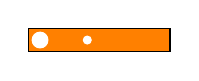
\begin{tikzpicture}
  \draw [black,fill=orange] (1.8,0.3) rectangle (0,0);
  \draw [white,fill] (0.15,0.15) circle [radius=0.1];
  \draw [white,fill] (0.75,0.15) circle [radius=0.05];
\end{tikzpicture}
,
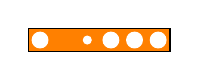
\begin{tikzpicture}
  \draw [black,fill=orange] (1.8,0.3) rectangle (0,0);
  \draw [white,fill] (0.15,0.15) circle [radius=0.1];
  \draw [white,fill] (0.75,0.15) circle [radius=0.05];
  \draw [white,fill] (1.05,0.15) circle [radius=0.1];
  \draw [white,fill] (1.35,0.15) circle [radius=0.1];
  \draw [white,fill] (1.65,0.15) circle [radius=0.1];
\end{tikzpicture}
und
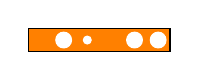
\begin{tikzpicture}
  \draw [black,fill=orange] (1.8,0.3) rectangle (0,0);
  \draw [white,fill] (0.45,0.15) circle [radius=0.1];
  \draw [white,fill] (0.75,0.15) circle [radius=0.05];
  \draw [white,fill] (1.35,0.15) circle [radius=0.1];
  \draw [white,fill] (1.65,0.15) circle [radius=0.1];
\end{tikzpicture}
interpretiert werden als 0(P), 7(U) und 27(G). Das kleine Führungsloch wird dabei benützt um den Lochstreifenleser in der richtigen Spur und Takt zu halten.\\

Der Lochenstreifenleser kann mit dem Befehl $I n$ bedient werden. Über die Lochstreifen wird das Programm mit beinhalten Daten an die Maschine übergeben. Außerdem kann eine Eingabe über den Teleprinter (Tastertur), mit dem Befehl $F n$ erfolgen.\\

\subsubsection{Ausgabewerk}



\subsection{Instruktionssatz}
In dem Instruktionssatz kann man erkennen, dass die meisten Befehle aus einem Funktionsteil (OP-Code) und einem numerischen Teil, der eine Speicheradresse angibt, bestehen. Nur einige Befehlen bestehen nur aus einem Funktionsteil, ohne Speicheradresse.\\
Insgesamt gibt es 18 Befehle mit der die ALU bedient, Werte aus dem Speicher in die Register geladen, Werte aus den Registern in den Speicher geladen, bedingte Sprünge ausgeführt werden können. Außerdem gibt es Befehle um die Ein- und Ausgabe zu steuern und einen Halt-Befehlt, der das Programm stoppt und die eingebaute Glocke läuten lässt.\\
\begin{table}
  \begin{tabularx}{\columnwidth}{|l|X|}
  \hline
  Name & Deschreibung\\ \hline
  $A n$ & Addiere den Wert in Speicherzelle n auf den Akkumulator.\\ \hline
  $S n$ & Substrahiere den Wert in Speicherzelle n von den Akkumulator.\\ \hline
  $H n$ & Kopiere den Wert in Speicherzelle n in den Akkumulator.\\ \hline
  $V n$ & Multipliziere den Wert in Speicherzelle n mit dem Wert im Multiplikationsregister und addiere das Resulat auf dem Akkumulator.\\ \hline
  $N n$ & Multipliziere den Wert in Speicherzelle n mit dem Wert im Multiplikationsregister und substrahiere das Resulat von dem Akkumulator.\\ \hline
  $T n$ & Kopiere den Wert im Akkumulator in die Speicherzelle n und lösche den Wert im Akkumulator.\\ \hline
  $U n$ & Kopiere den Wert im Akkumulator in die Speicherzelle n.\\ \hline
  $C n$ & Verunde die Speicherzelle n mit dem Multiplierregister.\\ \hline
  $R 2^{n-2}$ & Shifte den Wert im Akkumulator n Stellen nach rechts.\\ \hline
  $L 2^{n-2}$ & Shifte den Wert im Akkumulator n Stellen nach links.\\ \hline
  $E n$ & Falls der Wert im Akkumulator größer gleich 0 ist, setze die Ausführung an Speicherzelle n fort.\\ \hline
  $G n$ & Falls der Wert im Akkumulator kleiner als 0 ist, setze die Ausführung an Speicherzelle n fort.\\ \hline
  $I n$ & Ließ die nächsten 5 Bit vom Lochstreifen und Speichere sie in die niedrigwertigsten Bits in Speicherzelle n.\\ \hline
  $O n$ & Gibt den Buchstaben der den 5 höchstwertigen Bits in Speicherzelle n entspricht aus.\\ \hline
  $F n$ & Ließ die nächsten 5 Bit vom Teleprinter in die höchstwertigen Bits der Speicherzelle n.\\ \hline
  $X$ & Runde den Wert im Akkumulator auf 16 Bit.\\ \hline
  $Y$ & Runde den Wert im Akkumulator auf 34 Bit.\\ \hline
  $Z$ & Stoppe die Maschine und läute die Glocke.\\ \hline
  \end{tabularx}
\end{table}

\subsection{Speicher}

Der Speicher besteht aus Akustischen Verzögerungsleitungen. Es gibt 32 sogenannte Tanks, wobei 
jeder Tank etwa 1,5m lang ist und 32 Werte mit je 17 Bit speichern kann. Insgesamt können also
1024 Wörter gespeichert werden. ~\cite{theedsac}

\subsection{Order Sequence}

Die sogenannte order sequence (Ausführung von einem Befehl) ist in zwei Schritte unterteilt. Das Laden und das Ausführen des Befehls.

\subsubsection{Laden}
Im ersten Schritt wird der Befehlt aus der entsprechenden Speicherzelle im Hauptspeicher in das Befehlsregister (Ordertank) geladen.\\
Der Ordertank ist ein einzelner kürzerer Tank und kann genau einen Befehl speichern (18 Bit mit einem unbenüzten Bit). Die derzeitige Position im Programm ist ebenfalls in keim kurzen Tank, dem Befehlszähler (Sequence control tank), gespeichert. An dem Befehlszähler ist eine Additionsschaltung angeschlossen, die den Befehlszähler in jeder Befehlsausführung inkrementiert. Wenn ein Bedingungsbefehl $En$, oder $Gn$ geladen wird und die Bedingung wahr ist, wird der Befehlszähler nicht inkrementiert, sondern mit dem Adressfeld $n$ aus dem Befehl geladen.~\cite{theedsac}

\subsubsection{Ausführen}
Im zweiten Schritt, wird der geladene Befehl im Ordertank ausgeführt.~\cite{theedsac}

TODO: Anhand Datenbus Grafik, die beiden Schritte mit Beispielbefehl erklären.

\subsection{Datenbus}

Alle Bestandteile des Computers (Hauptspeicher, Arithmetische Einheit, Befehlsregister, Ein-/Ausgabewerk, usw.) sind mit sogenannten Gates verbunden.
Diese Gates können von zwei Einheiten gesteuert werden:
- Die Hauptsteuereinheit steht am Anfang der Maschine (TODO: Startet die Maschine...)
- Der sogenannte Order Interpreter schaltet die Gates entsprechend des ausgeführten Befehlt. (TODO: Grafik danach)
\subsection{Programmierung und Besonderheiten}

\subsubsection{Initial Orders}
Um das Programmieren zu erleichtern gab es in der Maschine ein Programm, die sogenannten initial orders, das beschrieb, wie ein Benutzerprogramm einzulesen war. Das Programm wandelte dann die Befehle des Benutzers, die in einer Art Assembler-Code geschrieben wurden, in ein für den Computer verständliches Programm um.\\

Das initial orders Programm besteht aus nur 31 Befehlen und ist fest verdrahtet auf motorisierten Wählscheiben gespeichert. Zu Beginn der Ausführung drehen sich diese Wählscheiben, und dass Programm wird in die Speicherzellen $m[0-30]$ geladen.\\

Die Hauptschleife der Initial Orders, beginnt bei Speicherzelle $m[6]$ mit $m[0-5]$ als Datenstellen. $m[0-5]$ werden wir folgt genützt.\\

In der Hauptschleife werden zuerst 5 Bit (OP-Code) vom Lochstreifen in den Akkumulator gelesen. Die Zahl wird dann in die obersten 5 Bit der Speicherzelle $m[0]$ geladen. Speicherstelle $m[1]$ ist jetzt leer.\\
Nun werden die nächsten 5 Bit in den Akkumulator geladen. Falls der Wert kleiner als 10 ist, handelt es sich um eine Zahl. Das Programm konvertiert den Buchstabencode nun in eine Binärzahl. Dies wird wiederholt, bis der geladene Wert größer gleich 10 ist.\\

Der Befehl in $m[25]$ ist in der Form $TnS$ (zu Beginn der Ausführung $T31S$) und wird benutzt, um eine Instruktion in $m[n]$ zu laden. Der Befehl wird von den Instruktionen 26-28 angepasst, sodass das Adressfeld um eins inkrementiert wird. In der nächsten Ausführung der Schleife wird dann also in die nächste Speicherstelle $m[n+1]$ geladen. 

Der erste Befehl auf jedem Lochstreifen muss immer $TnS$ lauten, wobei $n-1$ die letzte Adresse des Programms angibt.\\

\begin{table}
  \begin{tabular}{|l|l|p{5cm}|}
    \hline
      \# & Befehl & Kommentar \\
    \hline
      0 & $T0S$ & Daten: Hält das erste Zeichen des Befehls.\\ \hline
      1 & $H2S$ & Daten: Hält den Adressteil des Befehls.\\ \hline
      2 & $T0S$ & Daten\\ \hline
      3 & $E6S$ & Daten\\ \hline
      4 & $P1S$ & Daten\\ \hline
    5 & $ 5S$ & Daten: Konstante (10). Benötigt um nach Ende Adressteil zu prüfen.\\ \hline
    6 & $T0S$ &\\ \hline
    7 & $I0S$ &\\ \hline
    8 & $A0S$ &\\ \hline
    9 & $R16S$ &\\ \hline
    10 & $T0L$ &\\ \hline
    11 & $I2S$ &\\ \hline
    12 & $A2S$ &\\ \hline
    13 & $S5S$ &\\ \hline
    14 & $E21S$ &\\ \hline
    15 & $T3S$ &\\ \hline
    16 & $V1S$ &\\ \hline
    17 & $L8S$ &\\ \hline
    18 & $A2S$ &\\ \hline
    19 & $S5S$ &\\ \hline
    20 & $E11S$ &\\ \hline
    21 & $R4S$ &\\ \hline
    22 & $A1S$ &\\ \hline
    23 & $L0L$ &\\ \hline
    24 & $A0S$ &\\ \hline
    25 & $T(31)S$ &\\ \hline
    26 & $A25S$ &\\ \hline
    27 & $A4S$ &\\ \hline
    28 & $U25S$ &\\ \hline
    29 & $S31S$ &\\ \hline
    30 & $G6S$ &\\ \hline
  \end{tabular}
\end{table}

  

~\cite{theedsac}

\nocite{neumann,neumann1void,neumann2void,neumann3,neumann4}

\bibliographystyle{plain}
\bibliography{Latex-Einfuehrung}
\end{document}
